\documentclass[1p]{elsarticle_modified}
%\bibliographystyle{elsarticle-num}

%\usepackage[colorlinks]{hyperref}
%\usepackage{abbrmath_seonhwa} %\Abb, \Ascr, \Acal ,\Abf, \Afrak
\usepackage{amsfonts}
\usepackage{amssymb}
\usepackage{amsmath}
\usepackage{amsthm}
\usepackage{scalefnt}
\usepackage{amsbsy}
\usepackage{kotex}
\usepackage{caption}
\usepackage{subfig}
\usepackage{color}
\usepackage{graphicx}
\usepackage{xcolor} %% white, black, red, green, blue, cyan, magenta, yellow
\usepackage{float}
\usepackage{setspace}
\usepackage{hyperref}

\usepackage{tikz}
\usetikzlibrary{arrows}

\usepackage{multirow}
\usepackage{array} % fixed length table
\usepackage{hhline}

%%%%%%%%%%%%%%%%%%%%%
\makeatletter
\renewcommand*\env@matrix[1][\arraystretch]{%
	\edef\arraystretch{#1}%
	\hskip -\arraycolsep
	\let\@ifnextchar\new@ifnextchar
	\array{*\c@MaxMatrixCols c}}
\makeatother %https://tex.stackexchange.com/questions/14071/how-can-i-increase-the-line-spacing-in-a-matrix
%%%%%%%%%%%%%%%

\usepackage[normalem]{ulem}

\newcommand{\msout}[1]{\ifmmode\text{\sout{\ensuremath{#1}}}\else\sout{#1}\fi}
%SOURCE: \msout is \stkout macro in https://tex.stackexchange.com/questions/20609/strikeout-in-math-mode

\newcommand{\cancel}[1]{
	\ifmmode
	{\color{red}\msout{#1}}
	\else
	{\color{red}\sout{#1}}
	\fi
}

\newcommand{\add}[1]{
	{\color{blue}\uwave{#1}}
}

\newcommand{\replace}[2]{
	\ifmmode
	{\color{red}\msout{#1}}{\color{blue}\uwave{#2}}
	\else
	{\color{red}\sout{#1}}{\color{blue}\uwave{#2}}
	\fi
}

\newcommand{\Sol}{\mathcal{S}} %segment
\newcommand{\D}{D} %diagram
\newcommand{\A}{\mathcal{A}} %arc


%%%%%%%%%%%%%%%%%%%%%%%%%%%%%5 test

\def\sl{\operatorname{\textup{SL}}(2,\Cbb)}
\def\psl{\operatorname{\textup{PSL}}(2,\Cbb)}
\def\quan{\mkern 1mu \triangleright \mkern 1mu}

\theoremstyle{definition}
\newtheorem{thm}{Theorem}[section]
\newtheorem{prop}[thm]{Proposition}
\newtheorem{lem}[thm]{Lemma}
\newtheorem{ques}[thm]{Question}
\newtheorem{cor}[thm]{Corollary}
\newtheorem{defn}[thm]{Definition}
\newtheorem{exam}[thm]{Example}
\newtheorem{rmk}[thm]{Remark}
\newtheorem{alg}[thm]{Algorithm}

\newcommand{\I}{\sqrt{-1}}
\begin{document}

%\begin{frontmatter}
%
%\title{Boundary parabolic representations of knots up to 8 crossings}
%
%%% Group authors per affiliation:
%\author{Yunhi Cho} 
%\address{Department of Mathematics, University of Seoul, Seoul, Korea}
%\ead{yhcho@uos.ac.kr}
%
%
%\author{Seonhwa Kim} %\fnref{s_kim}}
%\address{Center for Geometry and Physics, Institute for Basic Science, Pohang, 37673, Korea}
%\ead{ryeona17@ibs.re.kr}
%
%\author{Hyuk Kim}
%\address{Department of Mathematical Sciences, Seoul National University, Seoul 08826, Korea}
%\ead{hyukkim@snu.ac.kr}
%
%\author{Seokbeom Yoon}
%\address{Department of Mathematical Sciences, Seoul National University, Seoul, 08826,  Korea}
%\ead{sbyoon15@snu.ac.kr}
%
%\begin{abstract}
%We find all boundary parabolic representation of knots up to 8 crossings.
%
%\end{abstract}
%\begin{keyword}
%    \MSC[2010] 57M25 
%\end{keyword}
%
%\end{frontmatter}

%\linenumbers
%\tableofcontents
%
\newcommand\colored[1]{\textcolor{white}{\rule[-0.35ex]{0.8em}{1.4ex}}\kern-0.8em\color{red} #1}%
%\newcommand\colored[1]{\textcolor{white}{ #1}\kern-2.17ex	\textcolor{white}{ #1}\kern-1.81ex	\textcolor{white}{ #1}\kern-2.15ex\color{red}#1	}

{\Large $\underline{12n_{0072}~(K12n_{0072})}$}

\setlength{\tabcolsep}{10pt}
\renewcommand{\arraystretch}{1.6}
\vspace{1cm}\begin{tabular}{m{100pt}>{\centering\arraybackslash}m{274pt}}
\multirow{5}{120pt}{
	\centering
	\includegraphics[width=112pt]{../../../GIT/diagram.site/Diagrams/png/2161_12n_0072.png}\\
\ \ \ A knot diagram\footnotemark}&
\allowdisplaybreaks
\textbf{Linearized knot diagam} \\
\cline{2-2}
 &
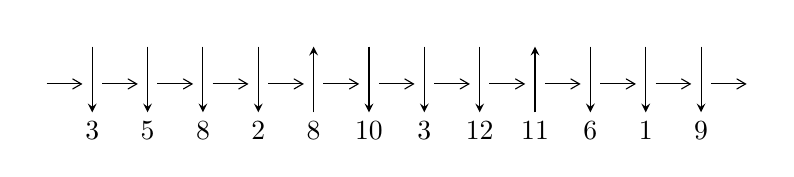
\begin{tikzpicture}[x=20pt, y=17pt]
	% nodes
	\node (C0) at (0, 0) {};
	\node (C1) at (1, 0) {};
	\node (C1U) at (1, +1) {};
	\node (C1D) at (1, -1) {3};

	\node (C2) at (2, 0) {};
	\node (C2U) at (2, +1) {};
	\node (C2D) at (2, -1) {5};

	\node (C3) at (3, 0) {};
	\node (C3U) at (3, +1) {};
	\node (C3D) at (3, -1) {8};

	\node (C4) at (4, 0) {};
	\node (C4U) at (4, +1) {};
	\node (C4D) at (4, -1) {2};

	\node (C5) at (5, 0) {};
	\node (C5U) at (5, +1) {};
	\node (C5D) at (5, -1) {8};

	\node (C6) at (6, 0) {};
	\node (C6U) at (6, +1) {};
	\node (C6D) at (6, -1) {10};

	\node (C7) at (7, 0) {};
	\node (C7U) at (7, +1) {};
	\node (C7D) at (7, -1) {3};

	\node (C8) at (8, 0) {};
	\node (C8U) at (8, +1) {};
	\node (C8D) at (8, -1) {12};

	\node (C9) at (9, 0) {};
	\node (C9U) at (9, +1) {};
	\node (C9D) at (9, -1) {11};

	\node (C10) at (10, 0) {};
	\node (C10U) at (10, +1) {};
	\node (C10D) at (10, -1) {6};

	\node (C11) at (11, 0) {};
	\node (C11U) at (11, +1) {};
	\node (C11D) at (11, -1) {1};

	\node (C12) at (12, 0) {};
	\node (C12U) at (12, +1) {};
	\node (C12D) at (12, -1) {9};
	\node (C13) at (13, 0) {};

	% arrows
	\draw[->,>={angle 60}]
	(C0) edge (C1) (C1) edge (C2) (C2) edge (C3) (C3) edge (C4) (C4) edge (C5) (C5) edge (C6) (C6) edge (C7) (C7) edge (C8) (C8) edge (C9) (C9) edge (C10) (C10) edge (C11) (C11) edge (C12) (C12) edge (C13) ;	\draw[->,>=stealth]
	(C1U) edge (C1D) (C2U) edge (C2D) (C3U) edge (C3D) (C4U) edge (C4D) (C5D) edge (C5U) (C6U) edge (C6D) (C7U) edge (C7D) (C8U) edge (C8D) (C9D) edge (C9U) (C10U) edge (C10D) (C11U) edge (C11D) (C12U) edge (C12D) ;
	\end{tikzpicture} \\
\hhline{~~} \\& 
\textbf{Solving Sequence} \\ \cline{2-2} 
 &
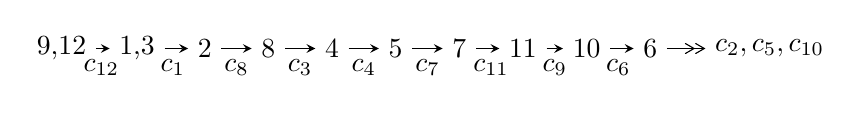
\begin{tikzpicture}[x=23pt, y=7pt]
	% node
	\node (A0) at (-1/8, 0) {9,12};
	\node (A1) at (17/16, 0) {1,3};
	\node (A2) at (17/8, 0) {2};
	\node (A3) at (25/8, 0) {8};
	\node (A4) at (33/8, 0) {4};
	\node (A5) at (41/8, 0) {5};
	\node (A6) at (49/8, 0) {7};
	\node (A7) at (57/8, 0) {11};
	\node (A8) at (65/8, 0) {10};
	\node (A9) at (73/8, 0) {6};
	\node (C1) at (1/2, -1) {$c_{12}$};
	\node (C2) at (13/8, -1) {$c_{1}$};
	\node (C3) at (21/8, -1) {$c_{8}$};
	\node (C4) at (29/8, -1) {$c_{3}$};
	\node (C5) at (37/8, -1) {$c_{4}$};
	\node (C6) at (45/8, -1) {$c_{7}$};
	\node (C7) at (53/8, -1) {$c_{11}$};
	\node (C8) at (61/8, -1) {$c_{9}$};
	\node (C9) at (69/8, -1) {$c_{6}$};
	\node (A10) at (11, 0) {$c_{2},c_{5},c_{10}$};

	% edge
	\draw[->,>=stealth]	
	(A0) edge (A1) (A1) edge (A2) (A2) edge (A3) (A3) edge (A4) (A4) edge (A5) (A5) edge (A6) (A6) edge (A7) (A7) edge (A8) (A8) edge (A9) ;
	\draw[->>,>={angle 60}]	
	(A9) edge (A10);
\end{tikzpicture} \\ 

\end{tabular} \\

\footnotetext{
The image of knot diagram is generated by the software ``\textbf{Draw programme}" developed by Andrew Bartholomew(\url{http://www.layer8.co.uk/maths/draw/index.htm\#Running-draw}), where we modified some parts for our purpose(\url{https://github.com/CATsTAILs/LinksPainter}).
}\phantom \\ \newline 
\centering \textbf{Ideals for irreducible components\footnotemark of $X_{\text{par}}$} 
 
\begin{align*}
I^u_{1}&=\langle 
2.81279\times10^{18} u^{59}-1.05287\times10^{19} u^{58}+\cdots+6.77112\times10^{17} b-1.27731\times10^{18},\\
\phantom{I^u_{1}}&\phantom{= \langle  }9.49759\times10^{17} u^{59}-1.92602\times10^{18} u^{58}+\cdots+6.77112\times10^{17} a-3.84134\times10^{17},\;u^{60}-5 u^{59}+\cdots+2 u+1\rangle \\
I^u_{2}&=\langle 
- u^8+u^7+u^6-2 u^5+u^3-2 u^2+b+u-1,\;- u^8+u^7+u^6-2 u^5+u^3-2 u^2+a+u-1,\\
\phantom{I^u_{2}}&\phantom{= \langle  }u^9- u^8-2 u^7+3 u^6+u^5-3 u^4+2 u^3- u+1\rangle \\
I^u_{3}&=\langle 
- a^2+b+a-1,\;a^3-2 a^2+a-1,\;u+1\rangle \\
\\
\end{align*}
\raggedright * 3 irreducible components of $\dim_{\mathbb{C}}=0$, with total 72 representations.\\
\footnotetext{All coefficients of polynomials are rational numbers. But the coefficients are sometimes approximated in decimal forms when there is not enough margin.}
\newpage
\renewcommand{\arraystretch}{1}
\centering \section*{I. $I^u_{1}= \langle 2.81\times10^{18} u^{59}-1.05\times10^{19} u^{58}+\cdots+6.77\times10^{17} b-1.28\times10^{18},\;9.50\times10^{17} u^{59}-1.93\times10^{18} u^{58}+\cdots+6.77\times10^{17} a-3.84\times10^{17},\;u^{60}-5 u^{59}+\cdots+2 u+1 \rangle$}
\flushleft \textbf{(i) Arc colorings}\\
\begin{tabular}{m{7pt} m{180pt} m{7pt} m{180pt} }
\flushright $a_{9}=$&$\begin{pmatrix}0\\u\end{pmatrix}$ \\
\flushright $a_{12}=$&$\begin{pmatrix}1\\0\end{pmatrix}$ \\
\flushright $a_{1}=$&$\begin{pmatrix}1\\u^2\end{pmatrix}$ \\
\flushright $a_{3}=$&$\begin{pmatrix}-1.40266 u^{59}+2.84446 u^{58}+\cdots-20.1139 u+0.567312\\-4.15409 u^{59}+15.5494 u^{58}+\cdots+1.51219 u+1.88640\end{pmatrix}$ \\
\flushright $a_{2}=$&$\begin{pmatrix}-4.29143 u^{59}+12.8571 u^{58}+\cdots-15.7514 u+0.224484\\-5.29000 u^{59}+18.1522 u^{58}+\cdots-3.12746 u+0.655392\end{pmatrix}$ \\
\flushright $a_{8}=$&$\begin{pmatrix}u\\u\end{pmatrix}$ \\
\flushright $a_{4}=$&$\begin{pmatrix}-1.47255 u^{59}+1.96750 u^{58}+\cdots-24.9698 u-0.484933\\-4.22398 u^{59}+14.6724 u^{58}+\cdots-3.34373 u+0.834159\end{pmatrix}$ \\
\flushright $a_{5}=$&$\begin{pmatrix}1.93062 u^{59}-6.99368 u^{58}+\cdots-6.44373 u+1.45359\\0.932046 u^{59}-1.69858 u^{58}+\cdots+6.18018 u+1.88449\end{pmatrix}$ \\
\flushright $a_{7}=$&$\begin{pmatrix}-1.88449 u^{59}+10.3545 u^{58}+\cdots+20.5308 u+2.41119\\2.65941 u^{59}-9.86960 u^{58}+\cdots-2.40765 u-1.93062\end{pmatrix}$ \\
\flushright $a_{11}=$&$\begin{pmatrix}- u^2+1\\- u^4\end{pmatrix}$ \\
\flushright $a_{10}=$&$\begin{pmatrix}u^5-2 u^3+u\\u^7- u^5+u\end{pmatrix}$ \\
\flushright $a_{6}=$&$\begin{pmatrix}-3.11073 u^{59}+10.8706 u^{58}+\cdots+6.04965 u-1.15134\\-2.11216 u^{59}+5.57554 u^{58}+\cdots-6.57426 u-1.58225\end{pmatrix}$\\&\end{tabular}
\flushleft \textbf{(ii) Obstruction class $= -1$}\\~\\
\flushleft \textbf{(iii) Cusp Shapes $= \frac{254104713520312101}{338556134519489602} u^{59}-\frac{287234417535105935}{338556134519489602} u^{58}+\cdots+\frac{9811882428269304349}{338556134519489602} u-\frac{403682827173379753}{169278067259744801}$}\\~\\
\newpage\renewcommand{\arraystretch}{1}
\flushleft \textbf{(iv) u-Polynomials at the component}\newline \\
\begin{tabular}{m{50pt}|m{274pt}}
Crossings & \hspace{64pt}u-Polynomials at each crossing \\
\hline $$\begin{aligned}c_{1}\end{aligned}$$&$\begin{aligned}
&u^{60}+17 u^{59}+\cdots+51 u+1
\end{aligned}$\\
\hline $$\begin{aligned}c_{2},c_{4}\end{aligned}$$&$\begin{aligned}
&u^{60}-11 u^{59}+\cdots+u+1
\end{aligned}$\\
\hline $$\begin{aligned}c_{3},c_{7}\end{aligned}$$&$\begin{aligned}
&u^{60}-2 u^{59}+\cdots-512 u-512
\end{aligned}$\\
\hline $$\begin{aligned}c_{5}\end{aligned}$$&$\begin{aligned}
&u^{60}+3 u^{59}+\cdots- u-1
\end{aligned}$\\
\hline $$\begin{aligned}c_{6},c_{10}\end{aligned}$$&$\begin{aligned}
&u^{60}+2 u^{59}+\cdots-28 u-8
\end{aligned}$\\
\hline $$\begin{aligned}c_{8},c_{12}\end{aligned}$$&$\begin{aligned}
&u^{60}-5 u^{59}+\cdots+2 u+1
\end{aligned}$\\
\hline $$\begin{aligned}c_{9}\end{aligned}$$&$\begin{aligned}
&u^{60}-24 u^{59}+\cdots+336 u+64
\end{aligned}$\\
\hline $$\begin{aligned}c_{11}\end{aligned}$$&$\begin{aligned}
&u^{60}+31 u^{59}+\cdots+52 u+1
\end{aligned}$\\
\hline
\end{tabular}\\~\\
\newpage\renewcommand{\arraystretch}{1}
\flushleft \textbf{(v) Riley Polynomials at the component}\newline \\
\begin{tabular}{m{50pt}|m{274pt}}
Crossings & \hspace{64pt}Riley Polynomials at each crossing \\
\hline $$\begin{aligned}c_{1}\end{aligned}$$&$\begin{aligned}
&y^{60}+63 y^{59}+\cdots-259 y+1
\end{aligned}$\\
\hline $$\begin{aligned}c_{2},c_{4}\end{aligned}$$&$\begin{aligned}
&y^{60}-17 y^{59}+\cdots-51 y+1
\end{aligned}$\\
\hline $$\begin{aligned}c_{3},c_{7}\end{aligned}$$&$\begin{aligned}
&y^{60}+60 y^{59}+\cdots+262144 y+262144
\end{aligned}$\\
\hline $$\begin{aligned}c_{5}\end{aligned}$$&$\begin{aligned}
&y^{60}-69 y^{59}+\cdots-55 y+1
\end{aligned}$\\
\hline $$\begin{aligned}c_{6},c_{10}\end{aligned}$$&$\begin{aligned}
&y^{60}+24 y^{59}+\cdots-336 y+64
\end{aligned}$\\
\hline $$\begin{aligned}c_{8},c_{12}\end{aligned}$$&$\begin{aligned}
&y^{60}-31 y^{59}+\cdots-52 y+1
\end{aligned}$\\
\hline $$\begin{aligned}c_{9}\end{aligned}$$&$\begin{aligned}
&y^{60}+20 y^{59}+\cdots-486656 y+4096
\end{aligned}$\\
\hline $$\begin{aligned}c_{11}\end{aligned}$$&$\begin{aligned}
&y^{60}+y^{59}+\cdots-1872 y+1
\end{aligned}$\\
\hline
\end{tabular}\\~\\
\newpage\flushleft \textbf{(vi) Complex Volumes and Cusp Shapes}
$$\begin{array}{c|c|c}  
\text{Solutions to }I^u_{1}& \I (\text{vol} + \sqrt{-1}CS) & \text{Cusp shape}\\
 \hline 
\begin{aligned}
u &= \phantom{-}0.337858 + 0.894600 I \\
a &= \phantom{-}0.13383 + 1.43636 I \\
b &= -1.48207 + 0.70345 I\end{aligned}
 & \phantom{-}7.94883 + 2.76650 I & -3.24347 - 1.05730 I \\ \hline\begin{aligned}
u &= \phantom{-}0.337858 - 0.894600 I \\
a &= \phantom{-}0.13383 - 1.43636 I \\
b &= -1.48207 - 0.70345 I\end{aligned}
 & \phantom{-}7.94883 - 2.76650 I & -3.24347 + 1.05730 I \\ \hline\begin{aligned}
u &= \phantom{-}0.275210 + 0.913906 I \\
a &= -0.05027 - 1.70048 I \\
b &= \phantom{-}1.38687 - 0.67504 I\end{aligned}
 & \phantom{-}6.81572 + 9.76098 I & -4.86985 - 5.65372 I \\ \hline\begin{aligned}
u &= \phantom{-}0.275210 - 0.913906 I \\
a &= -0.05027 + 1.70048 I \\
b &= \phantom{-}1.38687 + 0.67504 I\end{aligned}
 & \phantom{-}6.81572 - 9.76098 I & -4.86985 + 5.65372 I \\ \hline\begin{aligned}
u &= -0.933032\phantom{ +0.000000I} \\
a &= \phantom{-}4.22833\phantom{ +0.000000I} \\
b &= \phantom{-}4.57203\phantom{ +0.000000I}\end{aligned}
 & -3.01686\phantom{ +0.000000I} & -67.5230\phantom{ +0.000000I} \\ \hline\begin{aligned}
u &= \phantom{-}0.888711 + 0.272847 I \\
a &= -0.078190 - 0.558523 I \\
b &= \phantom{-}0.405126 + 0.581562 I\end{aligned}
 & \phantom{-}1.58683 - 3.66181 I & -4.28823 + 9.48383 I \\ \hline\begin{aligned}
u &= \phantom{-}0.888711 - 0.272847 I \\
a &= -0.078190 + 0.558523 I \\
b &= \phantom{-}0.405126 - 0.581562 I\end{aligned}
 & \phantom{-}1.58683 + 3.66181 I & -4.28823 - 9.48383 I \\ \hline\begin{aligned}
u &= \phantom{-}0.925197 + 0.542464 I \\
a &= \phantom{-}0.489920 - 0.539197 I \\
b &= \phantom{-}0.407019 + 0.364942 I\end{aligned}
 & \phantom{-}1.95619 - 3.10505 I & \phantom{-0.000000 -}0. + 4.26282 I \\ \hline\begin{aligned}
u &= \phantom{-}0.925197 - 0.542464 I \\
a &= \phantom{-}0.489920 + 0.539197 I \\
b &= \phantom{-}0.407019 - 0.364942 I\end{aligned}
 & \phantom{-}1.95619 + 3.10505 I & \phantom{-0.000000 } 0. - 4.26282 I \\ \hline\begin{aligned}
u &= \phantom{-}0.775160 + 0.782039 I \\
a &= \phantom{-}1.08347 - 1.85556 I \\
b &= \phantom{-}2.09668 - 0.60592 I\end{aligned}
 & \phantom{-}10.65710 + 0.79828 I & \phantom{-0.000000 } 0\\
 \hline 
 \end{array}$$\newpage$$\begin{array}{c|c|c}  
\text{Solutions to }I^u_{1}& \I (\text{vol} + \sqrt{-1}CS) & \text{Cusp shape}\\
 \hline 
\begin{aligned}
u &= \phantom{-}0.775160 - 0.782039 I \\
a &= \phantom{-}1.08347 + 1.85556 I \\
b &= \phantom{-}2.09668 + 0.60592 I\end{aligned}
 & \phantom{-}10.65710 - 0.79828 I & \phantom{-0.000000 } 0 \\ \hline\begin{aligned}
u &= \phantom{-}0.639144 + 0.625775 I \\
a &= \phantom{-}0.407955 + 0.337968 I \\
b &= -0.642419 + 0.534726 I\end{aligned}
 & \phantom{-}2.79847 - 1.51236 I & -1.81428 + 3.54798 I \\ \hline\begin{aligned}
u &= \phantom{-}0.639144 - 0.625775 I \\
a &= \phantom{-}0.407955 - 0.337968 I \\
b &= -0.642419 - 0.534726 I\end{aligned}
 & \phantom{-}2.79847 + 1.51236 I & -1.81428 - 3.54798 I \\ \hline\begin{aligned}
u &= \phantom{-}1.053880 + 0.334060 I \\
a &= \phantom{-}0.281699 + 0.729493 I \\
b &= \phantom{-}0.305612 - 0.503382 I\end{aligned}
 & \phantom{-}0.75501 + 1.63619 I & \phantom{-0.000000 } 0 \\ \hline\begin{aligned}
u &= \phantom{-}1.053880 - 0.334060 I \\
a &= \phantom{-}0.281699 - 0.729493 I \\
b &= \phantom{-}0.305612 + 0.503382 I\end{aligned}
 & \phantom{-}0.75501 - 1.63619 I & \phantom{-0.000000 } 0 \\ \hline\begin{aligned}
u &= -1.042430 + 0.414082 I \\
a &= -0.353731 - 1.109550 I \\
b &= -1.17215 - 1.41693 I\end{aligned}
 & -2.88310 + 2.96934 I & \phantom{-0.000000 } 0 \\ \hline\begin{aligned}
u &= -1.042430 - 0.414082 I \\
a &= -0.353731 + 1.109550 I \\
b &= -1.17215 + 1.41693 I\end{aligned}
 & -2.88310 - 2.96934 I & \phantom{-0.000000 } 0 \\ \hline\begin{aligned}
u &= -1.085610 + 0.332010 I \\
a &= -1.27018 - 2.13218 I \\
b &= -1.40022 - 1.45408 I\end{aligned}
 & -4.66678 + 1.12394 I & \phantom{-0.000000 } 0 \\ \hline\begin{aligned}
u &= -1.085610 - 0.332010 I \\
a &= -1.27018 + 2.13218 I \\
b &= -1.40022 + 1.45408 I\end{aligned}
 & -4.66678 - 1.12394 I & \phantom{-0.000000 } 0 \\ \hline\begin{aligned}
u &= \phantom{-}0.844243 + 0.760095 I \\
a &= -1.12133 + 1.75611 I \\
b &= -2.35320 + 0.80071 I\end{aligned}
 & \phantom{-}10.45220 - 6.50197 I & \phantom{-0.000000 } 0\\
 \hline 
 \end{array}$$\newpage$$\begin{array}{c|c|c}  
\text{Solutions to }I^u_{1}& \I (\text{vol} + \sqrt{-1}CS) & \text{Cusp shape}\\
 \hline 
\begin{aligned}
u &= \phantom{-}0.844243 - 0.760095 I \\
a &= -1.12133 - 1.75611 I \\
b &= -2.35320 - 0.80071 I\end{aligned}
 & \phantom{-}10.45220 + 6.50197 I & \phantom{-0.000000 } 0 \\ \hline\begin{aligned}
u &= -1.141290 + 0.233441 I \\
a &= \phantom{-}1.112610 + 0.300698 I \\
b &= \phantom{-}1.85544 + 0.38885 I\end{aligned}
 & -3.30337 - 0.69653 I & \phantom{-0.000000 } 0 \\ \hline\begin{aligned}
u &= -1.141290 - 0.233441 I \\
a &= \phantom{-}1.112610 - 0.300698 I \\
b &= \phantom{-}1.85544 - 0.38885 I\end{aligned}
 & -3.30337 + 0.69653 I & \phantom{-0.000000 } 0 \\ \hline\begin{aligned}
u &= -1.035450 + 0.539611 I \\
a &= \phantom{-}2.13511 + 1.38666 I \\
b &= \phantom{-}2.82243 + 0.20160 I\end{aligned}
 & \phantom{-}3.27029 + 1.99564 I & \phantom{-0.000000 } 0 \\ \hline\begin{aligned}
u &= -1.035450 - 0.539611 I \\
a &= \phantom{-}2.13511 - 1.38666 I \\
b &= \phantom{-}2.82243 - 0.20160 I\end{aligned}
 & \phantom{-}3.27029 - 1.99564 I & \phantom{-0.000000 } 0 \\ \hline\begin{aligned}
u &= \phantom{-}0.325660 + 0.762789 I \\
a &= \phantom{-}0.550531 - 1.183860 I \\
b &= \phantom{-}0.204288 + 0.081198 I\end{aligned}
 & \phantom{-}1.25130 + 3.50817 I & -4.71158 - 4.55526 I \\ \hline\begin{aligned}
u &= \phantom{-}0.325660 - 0.762789 I \\
a &= \phantom{-}0.550531 + 1.183860 I \\
b &= \phantom{-}0.204288 - 0.081198 I\end{aligned}
 & \phantom{-}1.25130 - 3.50817 I & -4.71158 + 4.55526 I \\ \hline\begin{aligned}
u &= \phantom{-}1.058140 + 0.503774 I \\
a &= \phantom{-}0.862782 - 0.336531 I \\
b &= \phantom{-}1.78762 - 0.38804 I\end{aligned}
 & -2.23222 - 3.63610 I & \phantom{-0.000000 } 0 \\ \hline\begin{aligned}
u &= \phantom{-}1.058140 - 0.503774 I \\
a &= \phantom{-}0.862782 + 0.336531 I \\
b &= \phantom{-}1.78762 + 0.38804 I\end{aligned}
 & -2.23222 + 3.63610 I & \phantom{-0.000000 } 0 \\ \hline\begin{aligned}
u &= -1.096800 + 0.538710 I \\
a &= -2.26195 - 1.34848 I \\
b &= -3.18815 - 0.39611 I\end{aligned}
 & \phantom{-}2.24129 + 8.72496 I & \phantom{-0.000000 } 0\\
 \hline 
 \end{array}$$\newpage$$\begin{array}{c|c|c}  
\text{Solutions to }I^u_{1}& \I (\text{vol} + \sqrt{-1}CS) & \text{Cusp shape}\\
 \hline 
\begin{aligned}
u &= -1.096800 - 0.538710 I \\
a &= -2.26195 + 1.34848 I \\
b &= -3.18815 + 0.39611 I\end{aligned}
 & \phantom{-}2.24129 - 8.72496 I & \phantom{-0.000000 } 0 \\ \hline\begin{aligned}
u &= \phantom{-}1.103150 + 0.529889 I \\
a &= -0.90009 + 1.69435 I \\
b &= -1.069960 + 0.856532 I\end{aligned}
 & -3.28631 - 6.19021 I & \phantom{-0.000000 } 0 \\ \hline\begin{aligned}
u &= \phantom{-}1.103150 - 0.529889 I \\
a &= -0.90009 - 1.69435 I \\
b &= -1.069960 - 0.856532 I\end{aligned}
 & -3.28631 + 6.19021 I & \phantom{-0.000000 } 0 \\ \hline\begin{aligned}
u &= \phantom{-}0.096441 + 0.769173 I \\
a &= \phantom{-}0.709332 + 0.054966 I \\
b &= -0.1034940 - 0.0442376 I\end{aligned}
 & -1.35021 + 2.66631 I & -2.81466 - 3.68602 I \\ \hline\begin{aligned}
u &= \phantom{-}0.096441 - 0.769173 I \\
a &= \phantom{-}0.709332 - 0.054966 I \\
b &= -0.1034940 + 0.0442376 I\end{aligned}
 & -1.35021 - 2.66631 I & -2.81466 + 3.68602 I \\ \hline\begin{aligned}
u &= -0.484975 + 0.602832 I \\
a &= \phantom{-}0.07018 - 2.49429 I \\
b &= -1.59748 - 1.32332 I\end{aligned}
 & \phantom{-}4.88218 + 2.55090 I & -5.75322 - 3.65479 I \\ \hline\begin{aligned}
u &= -0.484975 - 0.602832 I \\
a &= \phantom{-}0.07018 + 2.49429 I \\
b &= -1.59748 + 1.32332 I\end{aligned}
 & \phantom{-}4.88218 - 2.55090 I & -5.75322 + 3.65479 I \\ \hline\begin{aligned}
u &= -0.355933 + 0.652328 I \\
a &= -0.10224 + 2.47624 I \\
b &= \phantom{-}1.46844 + 1.04544 I\end{aligned}
 & \phantom{-}4.38705 - 4.06822 I & -6.35132 + 1.53091 I \\ \hline\begin{aligned}
u &= -0.355933 - 0.652328 I \\
a &= -0.10224 - 2.47624 I \\
b &= \phantom{-}1.46844 - 1.04544 I\end{aligned}
 & \phantom{-}4.38705 + 4.06822 I & -6.35132 - 1.53091 I \\ \hline\begin{aligned}
u &= \phantom{-}1.127800 + 0.566306 I \\
a &= -0.440646 + 0.632335 I \\
b &= -1.31378 + 1.01990 I\end{aligned}
 & -1.10174 - 8.51688 I & \phantom{-0.000000 } 0\\
 \hline 
 \end{array}$$\newpage$$\begin{array}{c|c|c}  
\text{Solutions to }I^u_{1}& \I (\text{vol} + \sqrt{-1}CS) & \text{Cusp shape}\\
 \hline 
\begin{aligned}
u &= \phantom{-}1.127800 - 0.566306 I \\
a &= -0.440646 - 0.632335 I \\
b &= -1.31378 - 1.01990 I\end{aligned}
 & -1.10174 + 8.51688 I & \phantom{-0.000000 } 0 \\ \hline\begin{aligned}
u &= -1.197690 + 0.405791 I \\
a &= \phantom{-}0.367973 - 0.288662 I \\
b &= \phantom{-}0.525918 - 0.753873 I\end{aligned}
 & -5.12612 + 1.38879 I & \phantom{-0.000000 } 0 \\ \hline\begin{aligned}
u &= -1.197690 - 0.405791 I \\
a &= \phantom{-}0.367973 + 0.288662 I \\
b &= \phantom{-}0.525918 + 0.753873 I\end{aligned}
 & -5.12612 - 1.38879 I & \phantom{-0.000000 } 0 \\ \hline\begin{aligned}
u &= \phantom{-}1.186970 + 0.490457 I \\
a &= \phantom{-}0.232541 + 0.230233 I \\
b &= \phantom{-}0.436907 + 0.672759 I\end{aligned}
 & -4.52134 - 7.29315 I & \phantom{-0.000000 } 0 \\ \hline\begin{aligned}
u &= \phantom{-}1.186970 - 0.490457 I \\
a &= \phantom{-}0.232541 - 0.230233 I \\
b &= \phantom{-}0.436907 - 0.672759 I\end{aligned}
 & -4.52134 + 7.29315 I & \phantom{-0.000000 } 0 \\ \hline\begin{aligned}
u &= \phantom{-}0.312115 + 0.635855 I \\
a &= \phantom{-}0.281014 - 0.263517 I \\
b &= \phantom{-}1.50466 - 0.17613 I\end{aligned}
 & -1.03251 + 1.61115 I & -5.03240 - 0.45414 I \\ \hline\begin{aligned}
u &= \phantom{-}0.312115 - 0.635855 I \\
a &= \phantom{-}0.281014 + 0.263517 I \\
b &= \phantom{-}1.50466 + 0.17613 I\end{aligned}
 & -1.03251 - 1.61115 I & -5.03240 + 0.45414 I \\ \hline\begin{aligned}
u &= -0.692437 + 0.039676 I \\
a &= \phantom{-}1.343570 + 0.174908 I \\
b &= \phantom{-}0.691006 + 0.039688 I\end{aligned}
 & -1.092530 + 0.001807 I & -8.18169 + 0.37203 I \\ \hline\begin{aligned}
u &= -0.692437 - 0.039676 I \\
a &= \phantom{-}1.343570 - 0.174908 I \\
b &= \phantom{-}0.691006 - 0.039688 I\end{aligned}
 & -1.092530 - 0.001807 I & -8.18169 - 0.37203 I \\ \hline\begin{aligned}
u &= -1.293890 + 0.191302 I \\
a &= \phantom{-}0.184711 + 0.635831 I \\
b &= \phantom{-}0.353270 - 0.535335 I\end{aligned}
 & \phantom{-}2.43582 + 0.64946 I & \phantom{-0.000000 } 0\\
 \hline 
 \end{array}$$\newpage$$\begin{array}{c|c|c}  
\text{Solutions to }I^u_{1}& \I (\text{vol} + \sqrt{-1}CS) & \text{Cusp shape}\\
 \hline 
\begin{aligned}
u &= -1.293890 - 0.191302 I \\
a &= \phantom{-}0.184711 - 0.635831 I \\
b &= \phantom{-}0.353270 + 0.535335 I\end{aligned}
 & \phantom{-}2.43582 - 0.64946 I & \phantom{-0.000000 } 0 \\ \hline\begin{aligned}
u &= \phantom{-}0.459124 + 0.506719 I \\
a &= -0.06558 + 1.82861 I \\
b &= \phantom{-}0.108857 + 0.574464 I\end{aligned}
 & -0.435329 - 0.564285 I & -6.58756 + 0.11639 I \\ \hline\begin{aligned}
u &= \phantom{-}0.459124 - 0.506719 I \\
a &= -0.06558 - 1.82861 I \\
b &= \phantom{-}0.108857 - 0.574464 I\end{aligned}
 & -0.435329 + 0.564285 I & -6.58756 - 0.11639 I \\ \hline\begin{aligned}
u &= \phantom{-}1.165420 + 0.613877 I \\
a &= \phantom{-}1.78237 - 1.00307 I \\
b &= \phantom{-}2.52278 + 0.05328 I\end{aligned}
 & \phantom{-}5.45561 - 8.29310 I & \phantom{-0.000000 } 0 \\ \hline\begin{aligned}
u &= \phantom{-}1.165420 - 0.613877 I \\
a &= \phantom{-}1.78237 + 1.00307 I \\
b &= \phantom{-}2.52278 - 0.05328 I\end{aligned}
 & \phantom{-}5.45561 + 8.29310 I & \phantom{-0.000000 } 0 \\ \hline\begin{aligned}
u &= -1.301730 + 0.255705 I \\
a &= \phantom{-}0.233918 - 0.675467 I \\
b &= \phantom{-}0.351604 + 0.513151 I\end{aligned}
 & \phantom{-}1.58747 - 5.92424 I & \phantom{-0.000000 } 0 \\ \hline\begin{aligned}
u &= -1.301730 - 0.255705 I \\
a &= \phantom{-}0.233918 + 0.675467 I \\
b &= \phantom{-}0.351604 - 0.513151 I\end{aligned}
 & \phantom{-}1.58747 + 5.92424 I & \phantom{-0.000000 } 0 \\ \hline\begin{aligned}
u &= \phantom{-}1.196470 + 0.595496 I \\
a &= -2.01101 + 0.96883 I \\
b &= -2.93963 + 0.12005 I\end{aligned}
 & \phantom{-}4.0303 - 15.2628 I & \phantom{-0.000000 } 0 \\ \hline\begin{aligned}
u &= \phantom{-}1.196470 - 0.595496 I \\
a &= -2.01101 - 0.96883 I \\
b &= -2.93963 - 0.12005 I\end{aligned}
 & \phantom{-}4.0303 + 15.2628 I & \phantom{-0.000000 } 0 \\ \hline\begin{aligned}
u &= -0.151881\phantom{ +0.000000I} \\
a &= \phantom{-}4.55507\phantom{ +0.000000I} \\
b &= \phantom{-}0.484061\phantom{ +0.000000I}\end{aligned}
 & -0.986470\phantom{ +0.000000I} & -9.89900\phantom{ +0.000000I}\\
 \hline 
 \end{array}$$\newpage\newpage\renewcommand{\arraystretch}{1}
\centering \section*{II. $I^u_{2}= \langle - u^8+u^7+u^6-2 u^5+u^3-2 u^2+b+u-1,\;- u^8+u^7+u^6-2 u^5+u^3-2 u^2+a+u-1,\;u^9- u^8-2 u^7+3 u^6+u^5-3 u^4+2 u^3- u+1 \rangle$}
\flushleft \textbf{(i) Arc colorings}\\
\begin{tabular}{m{7pt} m{180pt} m{7pt} m{180pt} }
\flushright $a_{9}=$&$\begin{pmatrix}0\\u\end{pmatrix}$ \\
\flushright $a_{12}=$&$\begin{pmatrix}1\\0\end{pmatrix}$ \\
\flushright $a_{1}=$&$\begin{pmatrix}1\\u^2\end{pmatrix}$ \\
\flushright $a_{3}=$&$\begin{pmatrix}u^8- u^7- u^6+2 u^5- u^3+2 u^2- u+1\\u^8- u^7- u^6+2 u^5- u^3+2 u^2- u+1\end{pmatrix}$ \\
\flushright $a_{2}=$&$\begin{pmatrix}u^8- u^7- u^6+2 u^5- u^3+2 u^2- u+2\\u^8- u^7- u^6+2 u^5- u^3+3 u^2- u+1\end{pmatrix}$ \\
\flushright $a_{8}=$&$\begin{pmatrix}u\\u\end{pmatrix}$ \\
\flushright $a_{4}=$&$\begin{pmatrix}u^8- u^7- u^6+2 u^5- u^3+2 u^2- u+1\\u^8- u^7- u^6+2 u^5- u^3+2 u^2- u+1\end{pmatrix}$ \\
\flushright $a_{5}=$&$\begin{pmatrix}-1\\- u^2\end{pmatrix}$ \\
\flushright $a_{7}=$&$\begin{pmatrix}u\\u\end{pmatrix}$ \\
\flushright $a_{11}=$&$\begin{pmatrix}- u^2+1\\- u^4\end{pmatrix}$ \\
\flushright $a_{10}=$&$\begin{pmatrix}u^5-2 u^3+u\\u^7- u^5+u\end{pmatrix}$ \\
\flushright $a_{6}=$&$\begin{pmatrix}- u^4+u^2-1\\- u^4\end{pmatrix}$\\&\end{tabular}
\flushleft \textbf{(ii) Obstruction class $= 1$}\\~\\
\flushleft \textbf{(iii) Cusp Shapes $= 3 u^8- u^7+u^5-4 u^4+5 u^3+7 u^2-4 u-6$}\\~\\
\newpage\renewcommand{\arraystretch}{1}
\flushleft \textbf{(iv) u-Polynomials at the component}\newline \\
\begin{tabular}{m{50pt}|m{274pt}}
Crossings & \hspace{64pt}u-Polynomials at each crossing \\
\hline $$\begin{aligned}c_{1},c_{2}\end{aligned}$$&$\begin{aligned}
&(u-1)^9
\end{aligned}$\\
\hline $$\begin{aligned}c_{3},c_{7}\end{aligned}$$&$\begin{aligned}
&u^9
\end{aligned}$\\
\hline $$\begin{aligned}c_{4}\end{aligned}$$&$\begin{aligned}
&(u+1)^9
\end{aligned}$\\
\hline $$\begin{aligned}c_{5},c_{9}\end{aligned}$$&$\begin{aligned}
&u^9+3 u^8+8 u^7+13 u^6+17 u^5+17 u^4+12 u^3+6 u^2+u-1
\end{aligned}$\\
\hline $$\begin{aligned}c_{6}\end{aligned}$$&$\begin{aligned}
&u^9+u^8+2 u^7+u^6+3 u^5+u^4+2 u^3+u-1
\end{aligned}$\\
\hline $$\begin{aligned}c_{8}\end{aligned}$$&$\begin{aligned}
&u^9+u^8-2 u^7-3 u^6+u^5+3 u^4+2 u^3- u-1
\end{aligned}$\\
\hline $$\begin{aligned}c_{10}\end{aligned}$$&$\begin{aligned}
&u^9- u^8+2 u^7- u^6+3 u^5- u^4+2 u^3+u+1
\end{aligned}$\\
\hline $$\begin{aligned}c_{11}\end{aligned}$$&$\begin{aligned}
&u^9-5 u^8+12 u^7-15 u^6+9 u^5+u^4-4 u^3+2 u^2+u-1
\end{aligned}$\\
\hline $$\begin{aligned}c_{12}\end{aligned}$$&$\begin{aligned}
&u^9- u^8-2 u^7+3 u^6+u^5-3 u^4+2 u^3- u+1
\end{aligned}$\\
\hline
\end{tabular}\\~\\
\newpage\renewcommand{\arraystretch}{1}
\flushleft \textbf{(v) Riley Polynomials at the component}\newline \\
\begin{tabular}{m{50pt}|m{274pt}}
Crossings & \hspace{64pt}Riley Polynomials at each crossing \\
\hline $$\begin{aligned}c_{1},c_{2},c_{4}\end{aligned}$$&$\begin{aligned}
&(y-1)^9
\end{aligned}$\\
\hline $$\begin{aligned}c_{3},c_{7}\end{aligned}$$&$\begin{aligned}
&y^9
\end{aligned}$\\
\hline $$\begin{aligned}c_{5},c_{9}\end{aligned}$$&$\begin{aligned}
&y^9+7 y^8+20 y^7+25 y^6+5 y^5-15 y^4+22 y^2+13 y-1
\end{aligned}$\\
\hline $$\begin{aligned}c_{6},c_{10}\end{aligned}$$&$\begin{aligned}
&y^9+3 y^8+8 y^7+13 y^6+17 y^5+17 y^4+12 y^3+6 y^2+y-1
\end{aligned}$\\
\hline $$\begin{aligned}c_{8},c_{12}\end{aligned}$$&$\begin{aligned}
&y^9-5 y^8+12 y^7-15 y^6+9 y^5+y^4-4 y^3+2 y^2+y-1
\end{aligned}$\\
\hline $$\begin{aligned}c_{11}\end{aligned}$$&$\begin{aligned}
&y^9- y^8+12 y^7-7 y^6+37 y^5+y^4-10 y^2+5 y-1
\end{aligned}$\\
\hline
\end{tabular}\\~\\
\newpage\flushleft \textbf{(vi) Complex Volumes and Cusp Shapes}
$$\begin{array}{c|c|c}  
\text{Solutions to }I^u_{2}& \I (\text{vol} + \sqrt{-1}CS) & \text{Cusp shape}\\
 \hline 
\begin{aligned}
u &= \phantom{-}0.772920 + 0.510351 I \\
a &= \phantom{-}0.624323 + 0.742839 I \\
b &= \phantom{-}0.624323 + 0.742839 I\end{aligned}
 & \phantom{-}0.13850 - 2.09337 I & -5.80108 + 4.26451 I \\ \hline\begin{aligned}
u &= \phantom{-}0.772920 - 0.510351 I \\
a &= \phantom{-}0.624323 - 0.742839 I \\
b &= \phantom{-}0.624323 - 0.742839 I\end{aligned}
 & \phantom{-}0.13850 + 2.09337 I & -5.80108 - 4.26451 I \\ \hline\begin{aligned}
u &= -0.825933\phantom{ +0.000000I} \\
a &= \phantom{-}3.14628\phantom{ +0.000000I} \\
b &= \phantom{-}3.14628\phantom{ +0.000000I}\end{aligned}
 & -2.84338\phantom{ +0.000000I} & -2.07210\phantom{ +0.000000I} \\ \hline\begin{aligned}
u &= -1.173910 + 0.391555 I \\
a &= -0.250943 - 1.026430 I \\
b &= -0.250943 - 1.026430 I\end{aligned}
 & -6.01628 + 1.33617 I & -17.3564 - 0.5967 I \\ \hline\begin{aligned}
u &= -1.173910 - 0.391555 I \\
a &= -0.250943 + 1.026430 I \\
b &= -0.250943 + 1.026430 I\end{aligned}
 & -6.01628 - 1.33617 I & -17.3564 + 0.5967 I \\ \hline\begin{aligned}
u &= \phantom{-}0.141484 + 0.739668 I \\
a &= \phantom{-}0.642765 + 0.088097 I \\
b &= \phantom{-}0.642765 + 0.088097 I\end{aligned}
 & -2.26187 + 2.45442 I & -11.99086 - 2.54651 I \\ \hline\begin{aligned}
u &= \phantom{-}0.141484 - 0.739668 I \\
a &= \phantom{-}0.642765 - 0.088097 I \\
b &= \phantom{-}0.642765 - 0.088097 I\end{aligned}
 & -2.26187 - 2.45442 I & -11.99086 + 2.54651 I \\ \hline\begin{aligned}
u &= \phantom{-}1.172470 + 0.500383 I \\
a &= -0.089286 + 0.842785 I \\
b &= -0.089286 + 0.842785 I\end{aligned}
 & -5.24306 - 7.08493 I & -15.8155 + 4.8919 I \\ \hline\begin{aligned}
u &= \phantom{-}1.172470 - 0.500383 I \\
a &= -0.089286 - 0.842785 I \\
b &= -0.089286 - 0.842785 I\end{aligned}
 & -5.24306 + 7.08493 I & -15.8155 - 4.8919 I\\
 \hline 
 \end{array}$$\newpage\newpage\renewcommand{\arraystretch}{1}
\centering \section*{III. $I^u_{3}= \langle - a^2+b+a-1,\;a^3-2 a^2+a-1,\;u+1 \rangle$}
\flushleft \textbf{(i) Arc colorings}\\
\begin{tabular}{m{7pt} m{180pt} m{7pt} m{180pt} }
\flushright $a_{9}=$&$\begin{pmatrix}0\\-1\end{pmatrix}$ \\
\flushright $a_{12}=$&$\begin{pmatrix}1\\0\end{pmatrix}$ \\
\flushright $a_{1}=$&$\begin{pmatrix}1\\1\end{pmatrix}$ \\
\flushright $a_{3}=$&$\begin{pmatrix}a\\a^2- a+1\end{pmatrix}$ \\
\flushright $a_{2}=$&$\begin{pmatrix}2\\a^2- a+1\end{pmatrix}$ \\
\flushright $a_{8}=$&$\begin{pmatrix}-1\\-1\end{pmatrix}$ \\
\flushright $a_{4}=$&$\begin{pmatrix}- a^2+3 a-1\\a\end{pmatrix}$ \\
\flushright $a_{5}=$&$\begin{pmatrix}- a^2+a+1\\0\end{pmatrix}$ \\
\flushright $a_{7}=$&$\begin{pmatrix}0\\a^2- a-1\end{pmatrix}$ \\
\flushright $a_{11}=$&$\begin{pmatrix}0\\-1\end{pmatrix}$ \\
\flushright $a_{10}=$&$\begin{pmatrix}0\\-1\end{pmatrix}$ \\
\flushright $a_{6}=$&$\begin{pmatrix}0\\a^2- a-1\end{pmatrix}$\\&\end{tabular}
\flushleft \textbf{(ii) Obstruction class $= 1$}\\~\\
\flushleft \textbf{(iii) Cusp Shapes $= a^2-2 a-7$}\\~\\
\newpage\renewcommand{\arraystretch}{1}
\flushleft \textbf{(iv) u-Polynomials at the component}\newline \\
\begin{tabular}{m{50pt}|m{274pt}}
Crossings & \hspace{64pt}u-Polynomials at each crossing \\
\hline $$\begin{aligned}c_{1},c_{3}\end{aligned}$$&$\begin{aligned}
&u^3- u^2+2 u-1
\end{aligned}$\\
\hline $$\begin{aligned}c_{2}\end{aligned}$$&$\begin{aligned}
&u^3+u^2-1
\end{aligned}$\\
\hline $$\begin{aligned}c_{4}\end{aligned}$$&$\begin{aligned}
&u^3- u^2+1
\end{aligned}$\\
\hline $$\begin{aligned}c_{5}\end{aligned}$$&$\begin{aligned}
&u^3+3 u^2+2 u-1
\end{aligned}$\\
\hline $$\begin{aligned}c_{6},c_{9},c_{10}\end{aligned}$$&$\begin{aligned}
&u^3
\end{aligned}$\\
\hline $$\begin{aligned}c_{7}\end{aligned}$$&$\begin{aligned}
&u^3+u^2+2 u+1
\end{aligned}$\\
\hline $$\begin{aligned}c_{8},c_{11}\end{aligned}$$&$\begin{aligned}
&(u-1)^3
\end{aligned}$\\
\hline $$\begin{aligned}c_{12}\end{aligned}$$&$\begin{aligned}
&(u+1)^3
\end{aligned}$\\
\hline
\end{tabular}\\~\\
\newpage\renewcommand{\arraystretch}{1}
\flushleft \textbf{(v) Riley Polynomials at the component}\newline \\
\begin{tabular}{m{50pt}|m{274pt}}
Crossings & \hspace{64pt}Riley Polynomials at each crossing \\
\hline $$\begin{aligned}c_{1},c_{3},c_{7}\end{aligned}$$&$\begin{aligned}
&y^3+3 y^2+2 y-1
\end{aligned}$\\
\hline $$\begin{aligned}c_{2},c_{4}\end{aligned}$$&$\begin{aligned}
&y^3- y^2+2 y-1
\end{aligned}$\\
\hline $$\begin{aligned}c_{5}\end{aligned}$$&$\begin{aligned}
&y^3-5 y^2+10 y-1
\end{aligned}$\\
\hline $$\begin{aligned}c_{6},c_{9},c_{10}\end{aligned}$$&$\begin{aligned}
&y^3
\end{aligned}$\\
\hline $$\begin{aligned}c_{8},c_{11},c_{12}\end{aligned}$$&$\begin{aligned}
&(y-1)^3
\end{aligned}$\\
\hline
\end{tabular}\\~\\
\newpage\flushleft \textbf{(vi) Complex Volumes and Cusp Shapes}
$$\begin{array}{c|c|c}  
\text{Solutions to }I^u_{3}& \I (\text{vol} + \sqrt{-1}CS) & \text{Cusp shape}\\
 \hline 
\begin{aligned}
u &= -1.00000\phantom{ +0.000000I} \\
a &= \phantom{-}0.122561 + 0.744862 I \\
b &= \phantom{-}0.337641 - 0.562280 I\end{aligned}
 & \phantom{-}1.37919 + 2.82812 I & -7.78492 - 1.30714 I \\ \hline\begin{aligned}
u &= -1.00000\phantom{ +0.000000I} \\
a &= \phantom{-}0.122561 - 0.744862 I \\
b &= \phantom{-}0.337641 + 0.562280 I\end{aligned}
 & \phantom{-}1.37919 - 2.82812 I & -7.78492 + 1.30714 I \\ \hline\begin{aligned}
u &= -1.00000\phantom{ +0.000000I} \\
a &= \phantom{-}1.75488\phantom{ +0.000000I} \\
b &= \phantom{-}2.32472\phantom{ +0.000000I}\end{aligned}
 & -2.75839\phantom{ +0.000000I} & -7.43020\phantom{ +0.000000I}\\
 \hline 
 \end{array}$$\newpage
\newpage\renewcommand{\arraystretch}{1}
\centering \section*{ IV. u-Polynomials}
\begin{tabular}{m{50pt}|m{274pt}}
Crossings & \hspace{64pt}u-Polynomials at each crossing \\
\hline $$\begin{aligned}c_{1}\end{aligned}$$&$\begin{aligned}
&((u-1)^9)(u^3- u^2+2 u-1)(u^{60}+17 u^{59}+\cdots+51 u+1)
\end{aligned}$\\
\hline $$\begin{aligned}c_{2}\end{aligned}$$&$\begin{aligned}
&((u-1)^9)(u^3+u^2-1)(u^{60}-11 u^{59}+\cdots+u+1)
\end{aligned}$\\
\hline $$\begin{aligned}c_{3}\end{aligned}$$&$\begin{aligned}
&u^9(u^3- u^2+2 u-1)(u^{60}-2 u^{59}+\cdots-512 u-512)
\end{aligned}$\\
\hline $$\begin{aligned}c_{4}\end{aligned}$$&$\begin{aligned}
&((u+1)^9)(u^3- u^2+1)(u^{60}-11 u^{59}+\cdots+u+1)
\end{aligned}$\\
\hline $$\begin{aligned}c_{5}\end{aligned}$$&$\begin{aligned}
&(u^3+3 u^2+2 u-1)\\
&\cdot(u^9+3 u^8+8 u^7+13 u^6+17 u^5+17 u^4+12 u^3+6 u^2+u-1)\\
&\cdot(u^{60}+3 u^{59}+\cdots- u-1)
\end{aligned}$\\
\hline $$\begin{aligned}c_{6}\end{aligned}$$&$\begin{aligned}
&u^3(u^9+u^8+2 u^7+u^6+3 u^5+u^4+2 u^3+u-1)\\
&\cdot(u^{60}+2 u^{59}+\cdots-28 u-8)
\end{aligned}$\\
\hline $$\begin{aligned}c_{7}\end{aligned}$$&$\begin{aligned}
&u^9(u^3+u^2+2 u+1)(u^{60}-2 u^{59}+\cdots-512 u-512)
\end{aligned}$\\
\hline $$\begin{aligned}c_{8}\end{aligned}$$&$\begin{aligned}
&(u-1)^3(u^9+u^8-2 u^7-3 u^6+u^5+3 u^4+2 u^3- u-1)\\
&\cdot(u^{60}-5 u^{59}+\cdots+2 u+1)
\end{aligned}$\\
\hline $$\begin{aligned}c_{9}\end{aligned}$$&$\begin{aligned}
&u^3(u^9+3 u^8+8 u^7+13 u^6+17 u^5+17 u^4+12 u^3+6 u^2+u-1)\\
&\cdot(u^{60}-24 u^{59}+\cdots+336 u+64)
\end{aligned}$\\
\hline $$\begin{aligned}c_{10}\end{aligned}$$&$\begin{aligned}
&u^3(u^9- u^8+2 u^7- u^6+3 u^5- u^4+2 u^3+u+1)\\
&\cdot(u^{60}+2 u^{59}+\cdots-28 u-8)
\end{aligned}$\\
\hline $$\begin{aligned}c_{11}\end{aligned}$$&$\begin{aligned}
&(u-1)^3(u^9-5 u^8+12 u^7-15 u^6+9 u^5+u^4-4 u^3+2 u^2+u-1)\\
&\cdot(u^{60}+31 u^{59}+\cdots+52 u+1)
\end{aligned}$\\
\hline $$\begin{aligned}c_{12}\end{aligned}$$&$\begin{aligned}
&(u+1)^3(u^9- u^8-2 u^7+3 u^6+u^5-3 u^4+2 u^3- u+1)\\
&\cdot(u^{60}-5 u^{59}+\cdots+2 u+1)
\end{aligned}$\\
\hline
\end{tabular}\newpage\renewcommand{\arraystretch}{1}
\centering \section*{ V. Riley Polynomials}
\begin{tabular}{m{50pt}|m{274pt}}
Crossings & \hspace{64pt}Riley Polynomials at each crossing \\
\hline $$\begin{aligned}c_{1}\end{aligned}$$&$\begin{aligned}
&((y-1)^9)(y^3+3 y^2+2 y-1)(y^{60}+63 y^{59}+\cdots-259 y+1)
\end{aligned}$\\
\hline $$\begin{aligned}c_{2},c_{4}\end{aligned}$$&$\begin{aligned}
&((y-1)^9)(y^3- y^2+2 y-1)(y^{60}-17 y^{59}+\cdots-51 y+1)
\end{aligned}$\\
\hline $$\begin{aligned}c_{3},c_{7}\end{aligned}$$&$\begin{aligned}
&y^9(y^3+3 y^2+2 y-1)(y^{60}+60 y^{59}+\cdots+262144 y+262144)
\end{aligned}$\\
\hline $$\begin{aligned}c_{5}\end{aligned}$$&$\begin{aligned}
&(y^3-5 y^2+10 y-1)\\
&\cdot(y^9+7 y^8+20 y^7+25 y^6+5 y^5-15 y^4+22 y^2+13 y-1)\\
&\cdot(y^{60}-69 y^{59}+\cdots-55 y+1)
\end{aligned}$\\
\hline $$\begin{aligned}c_{6},c_{10}\end{aligned}$$&$\begin{aligned}
&y^3(y^9+3 y^8+8 y^7+13 y^6+17 y^5+17 y^4+12 y^3+6 y^2+y-1)\\
&\cdot(y^{60}+24 y^{59}+\cdots-336 y+64)
\end{aligned}$\\
\hline $$\begin{aligned}c_{8},c_{12}\end{aligned}$$&$\begin{aligned}
&(y-1)^3(y^9-5 y^8+12 y^7-15 y^6+9 y^5+y^4-4 y^3+2 y^2+y-1)\\
&\cdot(y^{60}-31 y^{59}+\cdots-52 y+1)
\end{aligned}$\\
\hline $$\begin{aligned}c_{9}\end{aligned}$$&$\begin{aligned}
&y^3(y^9+7 y^8+20 y^7+25 y^6+5 y^5-15 y^4+22 y^2+13 y-1)\\
&\cdot(y^{60}+20 y^{59}+\cdots-486656 y+4096)
\end{aligned}$\\
\hline $$\begin{aligned}c_{11}\end{aligned}$$&$\begin{aligned}
&(y-1)^3(y^9- y^8+12 y^7-7 y^6+37 y^5+y^4-10 y^2+5 y-1)\\
&\cdot(y^{60}+y^{59}+\cdots-1872 y+1)
\end{aligned}$\\
\hline
\end{tabular}
\vskip 2pc
\end{document}